\section{Approach} 
\label{approach}

\subsection{Reinforcement Learning Method and Regression Model} 
\label{ch:approachA}

% TODO: The first section shall describe the reinforcement learning method and regression model you finally implemented, including all crucial design choices. You may also describe approaches you tried and abandoned later, including the reasons.

\subsubsection{Features}
\label{ch:approachAa}

This chapter describes how the game state is transformed into input features for the model. 
Our initial encoding is based on \cite{Kormelink2018}. The dictionary containing the game state is transformed into one vector, containing the input features.
Our input feature vector consists of the following five independent matrices:
\begin{itemize}
	\item Field state: free (0), breakable (1), obstructed cell (-1)
	\item Player position: player (1), otherwise(0)
	\item Opponent positions: opponent (1), otherwise(0)
	\item Danger level of position: danger (1), no danger (0) \newline
	Danger is caused by bombs on all fields an explosion can reach. Two aspects influence the value how dangerous a field is. The time until the bomb explodes and the distance from the bomb. We derived following equation for calculating the danger of a field for the field containing the bomb and the surrounding fields.
	
	$ danger = \frac{\frac{time\_Passed}{time\_needed\_to\_explode}}{\sqrt{distance}} $
	
	For example the bomb explodes after 4 time steps. Currently 2 time steps are over and the distance to the bomb is 3:
	
	$ danger = \frac{\frac{2}{4}}{\sqrt{2}} = 0.70 $
	
	TODO: normalized through equation
	TODO: advantage: gradation
	
	\item Desirability of position: desirable (1), not desirable (0)
\end{itemize}
These matrices are flattened and concatenated. This results in a feature vector containing 1445 elements (5*17*17).

Among other factors due to the high dimensionality the training process could be very slow. That is why the input state is further minimized.

TODO: adapt
\begin{itemize}
	\item Field state: free (0), breakable (1), obstructed cell (-1)
	\item Player position: player (1), otherwise(0)
	\item Opponent positions: opponent (1), otherwise(0)
	\item Danger level of position: danger (1), no danger (0)
	\item Desirability of position: desirable (1), not desirable (0)
\end{itemize}
These matrices are flattened and concatenated. This results in a feature vector containing 578 elements (2*17*17).


\subsubsection{Double Dueling DQN}
\label{ch:approachAb}



\subsection{Training process} 
\label{ch:approachB}

% TODO: The second section should describe your training process, including all tricks employed to speed it up (e.g. self play strategy, design of auxilliary rewards, prioritization of experience replay and so on).

\subsubsection{Exploration-Exploitation}
\label{ch:approachBa}

When choosing the right method for the exploration-exploitation tradeoff, \cite{Kormelink2018} gives an insight in how different exploration methods perform in the Bomberman environment (see \autoref{fig:exploration}). 

\begin{figure}[ht]
	\centering
	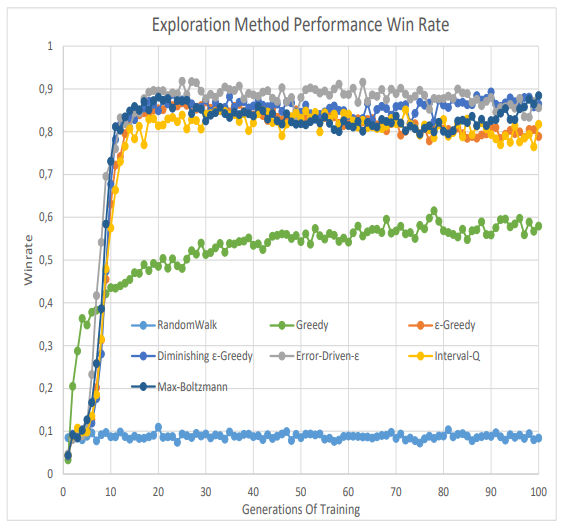
\includegraphics[width=0.6\linewidth]{figures/exploration.PNG}
	\caption{Comparison of different exploration methods}
	\label{fig:exploration}
\end{figure}

In the long run, Max Boltzmann performs best with 

\begin{equation}
	\Pi(s,a) = \frac{e^{Q(s,a)/T}}{\sum_i^{\abs{A}}e^{Q(s,a^i)/T}}
\end{equation}

and T being the temperature parameter. But as the result is based on 100 generations of training with each generation comprising 10.000 episodes, Diminishing $\epsilon$-Greedy as the second best exploration method was chosen as this exploration method converges faster in the early stages of training.

Two improvements where considered to optimize the exploration phase, but were discarded in the end. The first one is to replace the uniform sampling method by a multinomial sampling method in case an exploration step should be done, i.e. when a randomly generated number is smaller than $\epsilon$. This means the second best action would be chosen more often compared to other actions during the exploration phase. This could be beneficial especially in later phases of training in case the Q-values are close to each other. But esspecially in the beginning of the training phase this could lead towards an unintended bias towards specific actions as the exploration of others will be suppressed probabilistically.

The second improvement was to include an exploration function as \cite{Geron2018} proposes. A simple exploration function could be 

\begin{equation}
	f(q,n) = q + \frac{K}{1+n}
\end{equation}

with $q$ being the Q-value and $n$ being the count how often a specific action $a$ was chosen in state $s$. $K$ is a hyperparameter that determines the amount of curiosity during training. To implement this one would need to store $n$ for every state and action. But as the state is far too high dimensional in the Bomberman environment this would require a lot of training just as using the Max Boltzmann exploration method to be beneficial in the end. 

\subsubsection{Prioritized Experience Replay Buffer and SumTree}
\label{ch:approachBb}

Furthermore, a prioritized experience replay buffer was utilized to speed up the training process. To efficiently sample from it, a SumTree data structure was implemented inspired by \cite{Schaul2016}, which is a binary tree whose parent nodes store the sum of its children. All leaf nodes of the SumTree store the priority of each temporal difference error which is the L1-norm between two succeeding Q-values. The SumTree inherently offers a stratified sampling method to sample experiences with a high temporal difference error and therefore high priority more often. Therefore the leaf nodes are grouped into sum segments with a sum value greater or equal a threshold value. Each segment can therefore contain a different amount of leaf nodes as priorities often differ in their magnitude. The amount of segments is determined by the demanded batch size and the threshold value by dividing the total sum of the tree (stored in the root node) by the batch size. From each segment one priority is sampled uniformly. As high priorities have less competitors in their segment, they will be sampled more frequently until they get overwritten.  

\begin{figure}[ht]
	\centering
	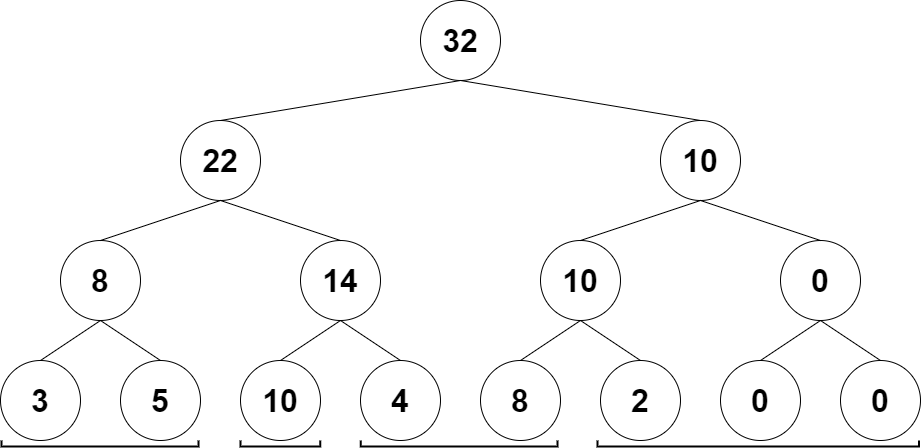
\includegraphics[width=0.6\linewidth]{figures/sumtree.PNG}
	\caption{Stratified sampling of priorities from a SumTree}
	\label{fig:sumtree}
\end{figure}

\autoref{fig:sumtree} illustrates the process of sampling priorities with a batch size of four. One can see that the priority with magnitude ten will be sampled every time as it is the only priority within the sum segment. One can also see that in case the prioritized experience replay buffer is not filled, zeros might be sampled. To counteract this, the amount of sum segments to divide the SumTree into is the batch size plus one. Adding values to the SumTree has the complexity O(n) whereas updating the SumTree has the complexity O(log n). 

The prioritized experience replay buffer only stores the priorities in the SumTree. The tuple $(s,a,r,s')$ is stored in a separate list. To access the according experience tuple for a priority, one can easily calculate the acording index by $index_{list} = index_{tree} - size_{per} + 1$. Note that \autoref{prio2} is used to calculate the priority value for each temporal difference error instead of \autoref{prio} as one would need to also sort the priorities in a different data structure which would add additional complexity and computing time. When sampling a batch from the prioritized experience replay buffer the tupel $(s,a,r,s')$, the according priorities, normalized weighting factors and update indices are returned. 

Drawbacks of using a prioritized experience replay buffer over a normal experience replay buffer is the continuous maintenance of the SumTree data structure, which is currently updated every training step, i.e. every step in an episode. Updated value changes need to be propagated to the root node. This adds additional computing time but the time gained in training progress by using prioritization should make up the time lost by maintaining the SumTree. Besides updating existing experiences every step also a new experience is added to the prioritized experience replay buffer every step which on the other hand executes fast. 

\subsubsection{Imitation Learning}
\label{ch:approachBc}

\subsubsection{Reward shaping}
\label{ch:approachBd}

Rewards are given when different kind of actions are taken or different kind of events occur. An overview of all rewards is given in \autoref{tab:rewards}.

\begin{table}[hbt!]
	\caption{Reward function}
	\label{tab:rewards}
	\begin{tabular}{|p{0.6\textwidth}|p{0.3\textwidth}|}
		\hline
		\textbf{Reward} & \textbf{Amount} \\ \hline
		Movement in/out of danger zone & -0.3/+0.3 \\ \hline
		Movement towards/away from nearest coin & +0.1/-0.1 \\ \hline
		WAITED & -0.2 \\ \hline
		INVALID\_ACTION & -1 \\ \hline
		BOMB\_DROPPED & 0.4 \\ \hline
		CRATE\_DESTROYED & 0.7 \\ \hline
		COIN\_COLLECTED & 0.2 \\ \hline
		KILLED\_OPPONENT & 1 \\ \hline
		KILLED\_SELF & -1 \\ \hline
		GOT\_KILLED & -1 \\ \hline
	\end{tabular}
\end{table}

Setting the rewards properly is a very difficult task and hard to evaluate without empirical study. Specifically for the Bomberman environment only for literatue was found that covers a reward function \cite{Kormelink2018, Franca2019}. All rewards are normalized to be in between -1 and 1 for more efficient training. Also focus was set on giving reward feedback as soon as possible to guide the training process better towards the desired behavior. 


In the first step the agent should be encouraged to gather coins, which is why the movement towards the nearest coin is rewarded. Nevertheless especially in the beginning of a game and also in late game phases setting bombs to find coins, to explore the arena and to kill opponents is even more crucial than finding coins. This is why the reward for dropping bombs is even higher than moving towards coins and gathering coins. To place bombs near creates the reward for destroying crates is set above the reward to simply dropping a bomb. 

Having this setup of arranging rewards leads to a lot of suicide of the agent in the very beginning of the training phase even if the the own agents death is punished. Therefore rewards for moving out of danger zones and punishments for moving in danger zones are given to encourage the agent to walk away from bombs dropped. Note that this reward is even higher than the movement reward towards the nearest coin to keep an agent out of a danger zone in case a coin is located in the bomb radius. 

Also an agent doing nothing or a invalid action should be punished by a negative reward. Therefore also no reward is given for rounds survived. Committing suicide or idleing was a big problem especially in the early stages of the training phase that should be counter using the introduced reward function. 

Killing opponents gives the highest reward, which is exactly five times higher than collecting a coin just like the points given inside the game.

Additional rewards could be given in case the agent gets closer to an opponent agent in case the agent does not commit enough to kill opponent agents during late game rounds. This still has to be evaluated.

\subsubsection{Hyperparameters}
\label{ch:approachBe}

\autoref{tab:hyperparameters} shows the choice of hyperparameters during training. As the computing resources are limited the hyperparameters were chosen to reach a fast convergence towards a first proper behavior which does not need to be optimal in the first place. \cite{Kormelink2018} states to train an agent over 100 generations à 10.000 episodes whereas the win rate in \autoref{fig:exploration} is already quite high just after 10 generations. Having 400 steps per episode 1.800 episodes can be trained locally within 24 hours which is really low inspite of using CUDA on a graphics card with a computing power score of 6.1 of 10. 

\begin{table}[hbt!]
	\caption{Hyperparameters}
	\label{tab:hyperparameters}
	\begin{tabular}{|p{0.6\textwidth}|p{0.3\textwidth}|}
		\hline
		\textbf{Hyperparameter} & \textbf{Value} \\ \hline
		Dense layer dimension & 128 \\ \hline
		\hline
		Activation function & ELU \\ \hline
		Loss function & Huber \\ \hline
		Learning rate & 0.01 \\ \hline
		\hline
		$\alpha$ & 0.65 \\ \hline
		$\beta$ & 0.4 \\ \hline
		$\beta$ increment & 0.00001 \\ \hline
		temporal difference $\epsilon$ bias & 0.01 \\ \hline
		\hline
		PER buffer min size & 8.192 \\ \hline
		PER buffer max size & 65.536 \\ \hline
		Batch size & 64 \\ \hline
		\hline
		$\gamma$ & 0.95 \\ \hline
		$\epsilon$ start & 0.3 \\ \hline
		$\epsilon$ end & 0.16 \\ \hline
		$\epsilon$ decay factor & 0.99999 \\ \hline
	\end{tabular}
\end{table}

The amount neurons per dense layer inside the dueling double DQN should not be higher than the input dimension itself as such a high degree of freedom is not needed to model the bomberman environment. For simplicity of the training process 128 was prefered over 256. 

The Exponential Linear Unit (ELU) activation function was chosen to fight the dead ReLU problem and to speed up training by pushing the mean activation towards zero and therefore decreasing the bias shift from ReLU. To be more robust towards outliers a Huber loss function was prefered over a conventional Squared Error loss function. The learning rate was set quite high with 0.01 to reach a fast convergence towards a first playable behavior on limited computing resources. 

The choice of the prioritized experience replay buffer hyperparameters was inspired by \cite{Schaul2016}. $\alpha$ was chosen slightly higher to once again speed up training through more prioritization. The $\beta$ increment summand was chosen just as high to converge $\beta$ to 1 at approximately the same time as $\epsilon$ converges to its lower limit after around 60.000 steps. 

The size of the prioritized experience replay buffer needs to be a power of two to result in a balanced SumTree. The batch size should be lower than one percent of the total prioritized experience replay buffer size, which is why the minimum size of the prioritized experience replay buffer was chosen to be 8192. This leads to a start of the training process after around 148 episodes. 

Choosing the right $\gamma$ in approximative Q-learningis not too important as future rewards are approximated. Using a decaying factor of $\gamma=0.95$ means rewards after 13 steps are only half that important as current rewards. $\epsilon$ is often decayed to around 0.05-0.2 and starts at either 1 or 0.3 \cite{Hessel2017, Kormelink2018, Franca2019}. To not have too much random behavior but setting more focus on fast behavior learning, 0.3 was chosen as the start value for $\epsilon$. 

Furthermore, the model and the  prioritized experience replay buffer are stored every 100 epsiodes in case the training process crashes because of unforeseen events. 

\subsubsection{Local Training Setup}
\label{ch:approachBf}

\subsubsection{Cloud Training and Training Visualization}
\label{ch:approachBg}

